\documentclass[30pt,twocolumn,letterpaper]{article}
\usepackage{cvpr}
\usepackage{times}
\usepackage{booktabs}
\usepackage{epsfig}
\usepackage{graphicx}
\usepackage{amsmath}
\usepackage{amssymb}
\cvprfinalcopy
\def\cvprPaperID{****}
\def\httilde{\mbox{\tt\raisebox{-.5ex}{\symbol{126}}}}
\usepackage{graphicx}
\usepackage{indentfirst}
\setlength{\parindent}{2em}
\usepackage{cite}
\usepackage[colorlinks,linkcolor=red,anchorcolor=blue,citecolor=green,backref=page]{hyperref}
\author{Qilei Zhang\\\\
Jul 12 2018}
\title{Manipulating potential wells in Logical Stochastic Resonance to obtain XOR logic}
\begin{document}
\maketitle
\begin{abstract}
  Logical random resonance (LSR) is an application of stochastic resonance in logical computation, that is, in the best noise, a nonlinear system driven by a weak signal that represents a logical input can produce logical output. The results obtained in a bistable system are extended to a number of stable dynamic systems that enable us to obtain XOR logic, in addition to the and (NAND) and OR (NOR) logic observed in the early study.
\end{abstract}
\section{Introduction}
With the continuous shrinking of electronic components and the advent of new computing paradigms like molecular or DNA computing systems where the influence of noise cannot be ignored are becoming commonplace. This problem is particularly evident in commonly used transistor based logic gates, where noise has been shown to actually bound the computing speed\cite{Bulsara2010Logical}. \\
\begin{figure}[htbp]
\small
\centering
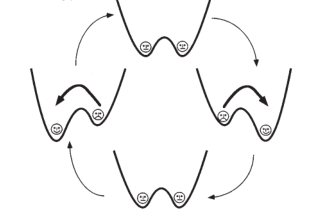
\includegraphics[width=20em]{000.png}
\caption{(a) Gradient F(x) + I for the three different values of I. (b) Potential energy U(x) + Ix for the three different values of I. It is evident that the stability of the wells
shifts depending on the input values. In both (a) and (b) we have �� = 1, �� = ?2.5, �� = 4.3 and K = 0.6.
}
\label{fig:lable}
\end{figure}\\
\section{Generalization to n-wells potential energy systems}
By analyzing the simplest cases, N stable potential energy systems are summed up to produce desired behavior, and the purpose is to summarize the models introduced and introduced in the previous section. That is to say, the three well potential is introduced, and its ability to generate XOR gates is demonstrated, and it is easy to reconfigure to get different logical outputs\cite{Storni2012Manipulating}.\\
\section{Conclusion}
In conclusion, in this study, a single system capable of producing robust XOR and NAND, OR and NOR logical behavior is provided\cite{Wang2014Logical}. It is important that the system can generate all these different logical behaviors without changing the underlying characteristics. This is contrary to the early implementation of LSR, in which the logic type is switched by changing the logic depth by changing the nonlinear characteristics of constant DC bias or changing the electric potential\cite{Zhang2013Effects}.\\
{\small
\bibliographystyle{ieee}
\bibliography{1}
}
\end{document}
